\documentclass[border=3pt]{standalone}
% Preâmbulo compartilhado pelos diagramas TikZ da aula 4 de Navegação (Representação de Mapas)
\usepackage[T1]{fontenc}
\usepackage[utf8]{inputenc}
\usepackage{lmodern}
\usepackage{amsmath}
\usepackage{xcolor}
\usepackage{tikz}
\usetikzlibrary{arrows.meta,angles,quotes,decorations.pathmorphing,decorations.pathreplacing,calc,
                positioning,shapes.geometric,shapes.misc,backgrounds,fit,
                math}

% Paleta (mesma dos SVGs originais)
\definecolor{dblue}{HTML}{2A5B8C}
\definecolor{dorange}{HTML}{B3541E}
\definecolor{dgreen}{HTML}{4A7C59}
\definecolor{dred}{HTML}{9C4B4B}
\definecolor{dcream}{HTML}{F4F1EA}
\definecolor{dshade}{HTML}{DDD7C9}

% Função gaussiana (não normalizada por padrão de escala visual)
\pgfmathdeclarefunction{gauss}{3}{%
  \pgfmathparse{1/(#3*sqrt(2*pi))*exp(-((#1-#2)^2)/(2*#3^2))}%
}

% Estilos comuns (prefixo d... para não colidir com chaves internas do pgf)
\tikzset{
  >={Stealth[length=2mm]},
  dguide/.style={gray!55, dashed, line width=0.4pt},
  daxis/.style={gray!60, line width=0.7pt, ->},
  dbody/.style={fill=black!3, draw=black!80, line width=1pt},
  dacc/.style={draw=dblue, line width=1pt},
  dlbl/.style={black!55, font=\small},
  dsub/.style={black!45, font=\footnotesize},
  dstate/.style={circle, draw=black!80, fill=dcream, line width=1pt,
                 minimum size=17mm, font=\large, inner sep=1pt},
  dobs/.style={circle, draw=black!80, fill=dshade, line width=1pt,
               minimum size=14mm, font=\large, inner sep=1pt},
  dbox/.style={rounded corners=2pt, draw=black!80, fill=dcream, line width=1pt,
               align=center, inner sep=6pt},
  dop/.style={circle, draw=black!80, fill=white, line width=1pt,
              minimum size=6mm, inner sep=0pt, font=\small},
  dtrans/.style={->, dblue, line width=1pt},
  dmeas/.style={->, dorange, line width=1pt},
  dcurve/.style={line width=1pt, dblue},
  dcurveb/.style={line width=1.4pt, dorange},
}

\begin{document}
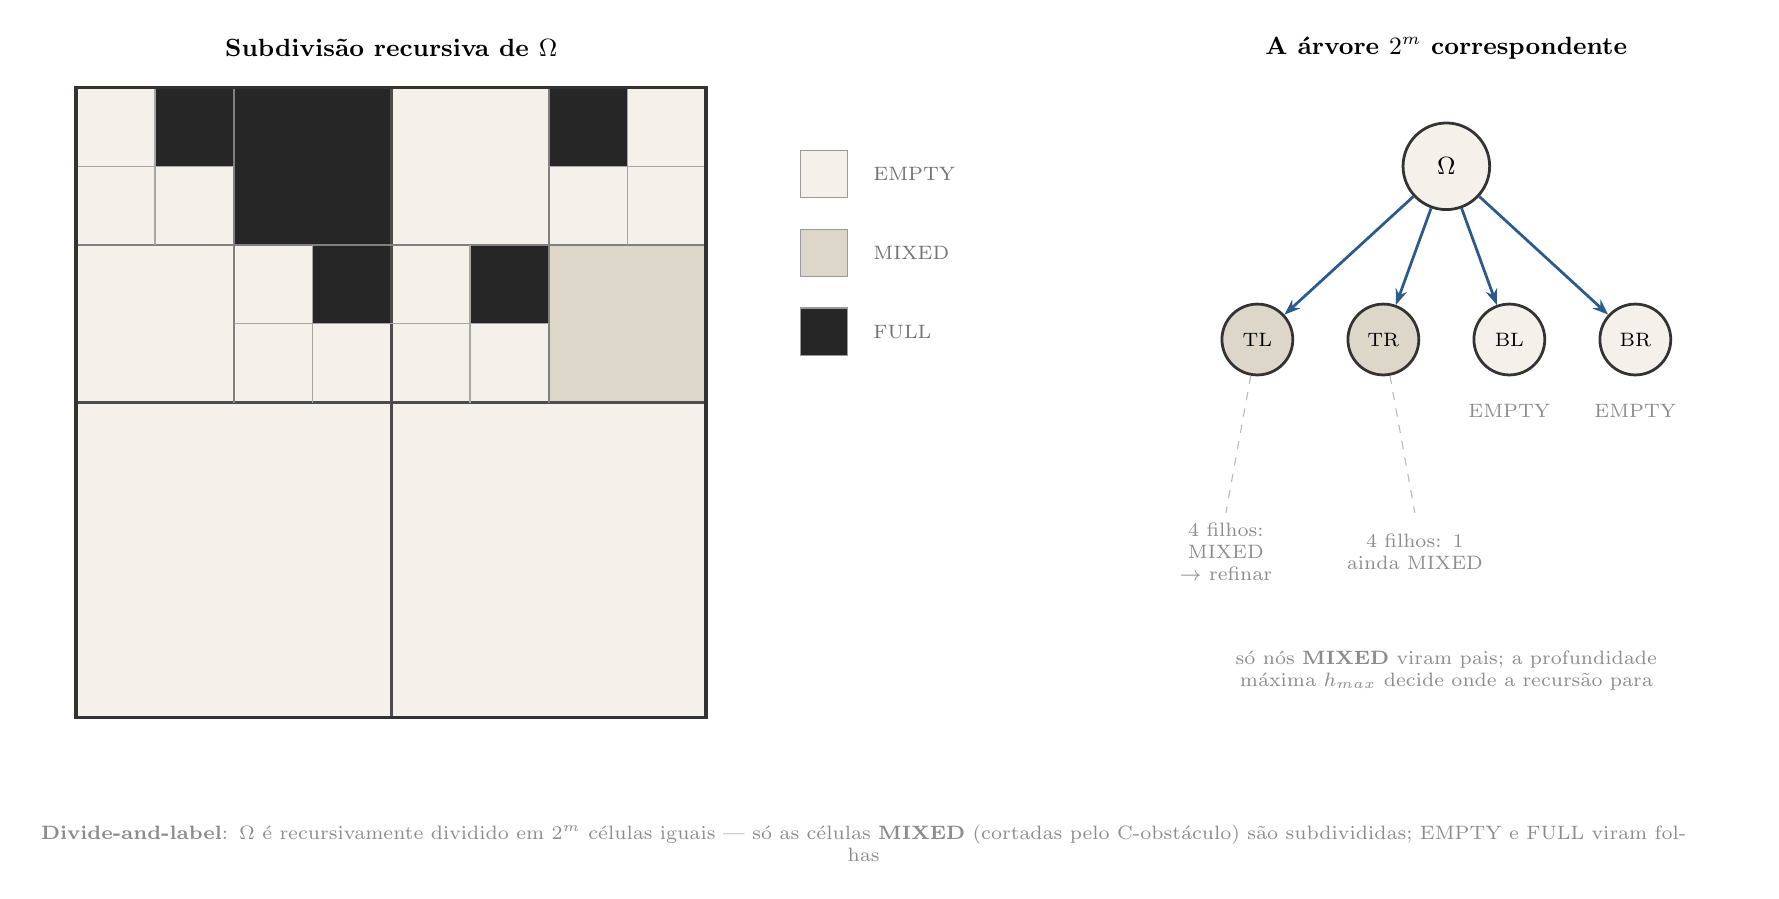
\begin{tikzpicture}[x=1cm,y=1cm]

  % ---------- Painel A: subdivisão espacial ----------
  \begin{scope}[shift={(0,0)}]
    \node[font=\bfseries\small] at (4,8.5) {Subdivisão recursiva de $\Omega$};

    % Fundo cheio: tudo começa como "livre" (EMPTY) por baixo
    \fill[dcream] (0,0) rectangle (8,8);

    % Nível 3 - folhas dentro de TLa [0,2]x[6,8]
    \fill[black!85] (1,7) rectangle (2,8);
    % Nível 3 - folhas dentro de TLd [2,4]x[4,6]
    \fill[black!85] (3,5) rectangle (4,6);
    % Nível 3 - folhas dentro de TRb [6,8]x[6,8]
    \fill[black!85] (6,7) rectangle (7,8);
    % Nível 3 - folhas dentro de TRc [4,6]x[4,6]
    \fill[black!85] (5,5) rectangle (6,6);

    % Nível 2 - FULL direto (TLb) e MIXED ainda não refinado (TRd)
    \fill[black!85] (2,6) rectangle (4,8);
    \fill[dshade] (6,4) rectangle (8,6);

    % ---- linhas da grade, por nível ----
    % nível 1
    \draw[black!70, line width=1pt] (4,0) -- (4,8);
    \draw[black!70, line width=1pt] (0,4) -- (8,4);
    % nível 2 (dentro de TL e TR)
    \draw[black!50, line width=0.6pt] (2,4) -- (2,8);
    \draw[black!50, line width=0.6pt] (0,6) -- (4,6);
    \draw[black!50, line width=0.6pt] (6,4) -- (6,8);
    \draw[black!50, line width=0.6pt] (4,6) -- (8,6);
    % nível 3 (dentro de TLa, TLd, TRb, TRc)
    \draw[black!35, line width=0.4pt] (1,6) -- (1,8);
    \draw[black!35, line width=0.4pt] (0,7) -- (2,7);
    \draw[black!35, line width=0.4pt] (3,4) -- (3,6);
    \draw[black!35, line width=0.4pt] (2,5) -- (4,5);
    \draw[black!35, line width=0.4pt] (7,6) -- (7,8);
    \draw[black!35, line width=0.4pt] (6,7) -- (8,7);
    \draw[black!35, line width=0.4pt] (5,4) -- (5,6);
    \draw[black!35, line width=0.4pt] (4,5) -- (6,5);

    \draw[draw=black!80, line width=1.3pt] (0,0) rectangle (8,8);

    % Legenda
    \begin{scope}[shift={(9.2,6.6)}]
      \fill[dcream] (0,0) rectangle (0.6,0.6); \draw[black!40,line width=0.4pt] (0,0) rectangle (0.6,0.6);
      \node[dlbl, anchor=west, font=\scriptsize] at (0.8,0.3) {EMPTY};
      \fill[dshade] (0,-1.0) rectangle (0.6,-0.4); \draw[black!40,line width=0.4pt] (0,-1.0) rectangle (0.6,-0.4);
      \node[dlbl, anchor=west, font=\scriptsize] at (0.8,-0.7) {MIXED};
      \fill[black!85] (0,-2.0) rectangle (0.6,-1.4); \draw[black!40,line width=0.4pt] (0,-2.0) rectangle (0.6,-1.4);
      \node[dlbl, anchor=west, font=\scriptsize] at (0.8,-1.7) {FULL};
    \end{scope}
  \end{scope}

  % ---------- Painel B: árvore (esquemática) ----------
  \begin{scope}[shift={(14.4,0)}]
    \node[font=\bfseries\small] at (3.0,8.5) {A árvore $2^m$ correspondente};

    \node[dstate, minimum size=11mm, font=\small] (root) at (3.0,7.0) {$\Omega$};

    \node[dobs, minimum size=9mm, fill=dshade, font=\scriptsize] (tl) at (0.6,4.8) {TL};
    \node[dobs, minimum size=9mm, fill=dshade, font=\scriptsize] (tr) at (2.2,4.8) {TR};
    \node[dobs, minimum size=9mm, fill=dcream, font=\scriptsize] (bl) at (3.8,4.8) {BL};
    \node[dobs, minimum size=9mm, fill=dcream, font=\scriptsize] (br) at (5.4,4.8) {BR};
    \draw[dtrans] (root) -- (tl);
    \draw[dtrans] (root) -- (tr);
    \draw[dtrans] (root) -- (bl);
    \draw[dtrans] (root) -- (br);
    \node[dsub, font=\scriptsize] at (3.8,3.9) {EMPTY};
    \node[dsub, font=\scriptsize] at (5.4,3.9) {EMPTY};

    \draw[dguide] (tl) -- (0.2,2.6);
    \draw[dguide] (tr) -- (2.6,2.6);
    \node[dsub, font=\scriptsize, align=center, text width=2.0cm] at (0.2,2.1) {4 filhos: MIXED $\to$ refinar};
    \node[dsub, font=\scriptsize, align=center, text width=2.0cm] at (2.6,2.1) {4 filhos: 1 ainda MIXED};

    \node[dsub, font=\scriptsize, align=center, text width=7.5cm] at (3.0,0.6)
       {só nós \textbf{MIXED} viram pais; a profundidade máxima $h_{max}$ decide onde a recursão para};
  \end{scope}

  \node[dsub, font=\scriptsize, align=center, text width=21cm] at (10,-1.6)
     {\textbf{Divide-and-label}: $\Omega$ é recursivamente dividido em $2^m$ células iguais --- só as células \textbf{MIXED} (cortadas pelo C-obstáculo) são subdivididas; EMPTY e FULL viram folhas};

\end{tikzpicture}
\end{document}
